%
% physik.tex -- Physikalische Eigenschaften des Klimasystems
%
% (c) 2018 Prof Dr Andreas Müller, Hochschule Rapperswil
%

\section{Physikalische Eigenschaften des Klimasystems\label{section:physik}}
In diesem Abschnitt stellen wir die physikalischen Eigenschaften
aller wesentlicher Komponenten des Klimasystems zusammen.
Dabei geht es zunächst nur darum, die grundlegende Physik in 
Erinnerung zu rufen und die Naturgesetze, die die Wechselwirkungen
zwischen den Komponenten beschreiben.
Auf die Details der mathematischen Modellierung der zukünftigen
Veränderung dieser Grössen werden wir erst später eingehen.

\subsection{Wärme, Konvektion, Kondensation}
Die wohl wichtigste Klima-Grösse ist die Temperatur.
Sie drückt aus, wieviel Energie in Form von Wärme ein Körper enthält.

\subsubsection{Wärmekapazität}
Die spezifische Wärme $C$ gibt an, wie die innere Energie sich bei
einer Temperaturänderung $\Delta T$ verändert:
\[
\Delta E = C\cdot\Delta T.
\]
Der Körper speichert Energie in Form der thermischen Bewegung der
einzelnen Atome.
Schwerere Atome können bei gleicher Bewegungsgeschwindigkeit 
mehr Energie speichern.
Stoffe mit grösserer Dichte können mehr Atome und damit auch mehr
Wärmeenergie in einem kleineren Volumen unterbringen.
Die spezifische Wärmekapazität $c$ gibt an, welche Wärmekapazität
ein Kilogramm eines Stoffes hat.
Ein Körper der Masse $m$ hat also die Wärmekapazität $C=cm$.

\subsubsection{Wärmeleitung}
Herrschen in einem Körper Temperaturunterschiede, ist $T$ nicht mehr
nur eine konstante, sondern eine Funktion der Koordinaten und auch der
Zeit.
Temperaturunterschiede werden sich ausgleichen, indem Energie von
wärmeren zu kälteren Teilen des Körpers fliegt.
Dies geschieht umso schneller, je grösser die Unterschiede sind.
Die Wärmeleitungsgleichung
\begin{equation}
\frac{\partial T}{\partial t}
=
\kappa
\biggl(
\frac{\partial^2}{\partial x^2}
+
\frac{\partial^2}{\partial y^2}
+
\frac{\partial^2}{\partial z^2}
\biggr)
T
\label{skript:waermeleitung}
\end{equation}
beschreibt die Entwicklung der Funktion $T(x,y,z,t)$ an jedem
Ort des Raumes \cite{skript:waermeleitung}.
Der Koeffizient $\kappa$ ist eine Materialkonstante, die beschreibt,
wie schnell sich die Temperaturunterschiede ausgleichen können.
Ist $\kappa=0$, folgt $\partial T/\partial t=0$, die Temperatur 
ändert sich nicht, es findet keine Wärmeleitung statt.

Die rechte Seite von \eqref{skript:waermeleitung} kann mit dem
sogenannten Laplace-Operator gemäss der folgenden Definition 
geschrieben werden.

\begin{definition}
Der Operator
\[
\Delta
=
\frac{\partial^2}{\partial x^2}
+
\frac{\partial^2}{\partial y^2}
+
\frac{\partial^2}{\partial z^2}
\]
heisst der
{\em Laplace-Operator}.
\end{definition}

Die Wärmeleitungsgleichung erhält damit die Form
\begin{equation}
\frac{\partial T}{\partial t}
=
\kappa\Delta T.
\label{skript:waermeleitung2}
\end{equation}

\subsubsection{Konvektion}
Wärmeleitung kann Wärmeenergie nur vergleichsweise langsam transportieren.
Das einleitende Beispiel des Kochtopfs zeigt auch, wie ein effizienterer
Energietransport funktionieren kann.
In der Atmosphäre dehnt sich warme Luft aus.
Dank der geringeren Dichte können warme Luftblasen aufsteigen und damit
Wärme viel effizienter in die obere Atmosphäre transportieren
als dies mit Wärmeleitung möglich wäre.
Dieser Prozess heisst {\em Konvektion} \cite{skript:konvektion}.
\index{Konvektion}%

Wir wollen den Fall eines strömenden Mediums mathematisch etwas genauer
ausarbeiten.
Bewegt sich das Medium mit der Geschwindigkeit $\vec v$, dann ändert sich
die Temperatur des Mediums, welches sich über dem Punkt $P=(x,y,z)$
befindet.
Nach der Zeit $\Delta t$ befindet sich derjenige Teil des Mediums
über dem Punkt $P$, der sich vorher über dem Punkt $P-\Delta t\cdot\vec v$
befand.
Die Temperatur zur Zeit $t+\Delta t$ ist daher
$T(P,t+\Delta t)=T(P-\Delta t,t)$.
Die Temperaturänderung
\begin{align*}
T(P,t+\Delta t)
&=
T(P,t) + (T(P,t+\Delta t)-T(P,t))
=
T(P,t) + T(P-\vec v\Delta t, t)-T(P,t)
\\
\frac{
T(P,t+\Delta t)
-
T(P,t)
}{\Delta t}
&=
\frac{
T(P-\vec v\Delta t, t)-T(P,t)
}{\Delta t}.
\end{align*}
Beim Grenzübergang $\Delta t\to 0$ wird aus der linken Seite die
partielle Ableitung nach $t$.
Die rechte Seite kann mit Hilfe der Kettenregel berechnet weren.
Es wird
\begin{equation}
\frac{\partial T}{\partial t}
=
-
\frac{\partial T}{\partial x} v_x
-
\frac{\partial T}{\partial y} v_y
-
\frac{\partial T}{\partial z} v_z.
\label{skript:advektion1}
\end{equation}
Der Ausdruck auf der rechten Seite kann vektoriell mit der folgenden
Definition etwas eleganter geschrieben werden.

\begin{definition}
Der vektorielle Operator 
\[
\nabla
=
\def\arraystretch{1.3}
\begin{pmatrix}
\frac{\partial}{\partial x}\\
\frac{\partial}{\partial y}\\
\frac{\partial}{\partial z}
\end{pmatrix}
\]
heisst der {\em Nabla-Operator}.
Der Vektor
\[
\nabla f
=
\def\arraystretch{1.3}
\begin{pmatrix}
\frac{\partial f}{\partial x}\\
\frac{\partial f}{\partial y}\\
\frac{\partial f}{\partial z}
\end{pmatrix}
=
\operatorname{grad} f
\]
heisst der {\em Gradient} von $f$.
\end{definition}
\index{Gradient}%
\index{Nabla-Operator}%

Die Temperaturänderung in Folge der Strämung 
\eqref{skript:advektion1}
wird 
\begin{equation}
\frac{\partial T}{\partial t}
=
-\vec{v}\cdot\nabla T.
\label{skript:advektion2}
\end{equation}
\index{Advektion}%
Man nennt diese Temperaturänderung durch die Strömung auch
{\em Advektion}.
Die Wärmeleitungsgleichung kann damit zu einem umfassenderen
Modell
\begin{equation}
\frac{\partial T}{\partial t}
=
-\vec{v}\cdot\nabla T +\kappa\Delta T
\label{skript:waermeleitungadvektion}
\end{equation}
zusammengefasst werden.
Es ist geeignet für die Beschreibung sowohl der Atmosphäre wie auch des
Wärmeaustausches in den Ozeanen.

\subsubsection{Phasenübergänge}
Um ein Kilogramm Wasser bei $20^\circ\text{C}$ zu verdunsten, ist eine
latente Wärme von $2480\,\text{kJ}$ nötig.
Um ein Kilogramm Luft um ein Grad zu erwärmen, sind dagegen nur
$1.005\,\text{kJ}$ notwendig.
Anders herum bedeutet dies, dass eine mit Wasserdampf angereicherte Atmosphäre
sehr viel mehr Energie in Form von latenter Wärme speichern kann, als
allein durch die Wärmekapazität trockener Luft möglich wäre.

Wir haben damit zwei Mechanismen identifiziert, wie eingestrahlte
und in der Erdkruste als Wärme gespeicherte Energie in die Atmosphäre 
transportiert werden kann.
Einerseits kann Luft über aufgewärmten Landmassen oder dem Meer erwärmt
werden und als Konvektionsströmung aufsteigen.
Andererseits kann Wasser an der Oberfläche verdampft werden damit die
latente Wärme in die Atmosphäre übergehen.
Man nennt diese Mechanismen auch turbulente Flüsse
\cite[S.~70]{skript:wiefunktioniertdas}.

Der Wassergehalt der Luft kann höchstens einige wenige Prozente betragen.
Zwar ist die Wärmespeicherung durch Verdunstung über 2000 mal effizienter,
aber weil nur wenig Wasser dafür zur Verfügung steht, übernimmt die Verdunstung
doch nicht einen derart grossen Teil des Energietransports von der
Oberfläche in die Atmosphäre.
In der Tat finden etwa 30\% des Energietransports von der Erdkruste
in die Atmosphäre durch turbulente Flüsse statt, davon etwa
7\% durch Konvektion und 23\% durch latente Wärme
\cite[S.~70]{skript:wiefunktioniertdas}.
Höhere Temperaturen begünstigen die Verdunstung und verschieben diesen
Anteil zugunsten der latenten Wärme.
Man darf also davon ausgehen, dass höhere Oberflächentemperaturen
zu einem überproportional höheren Energietransport in die Atmosphäre
führen.

In der Atmosphäre kann die Energie über grosse Distanzen transportiert
und später wieder freigesetzt werden, wie Hurricanes und Tornadoes
eindrücklich demonstrieren können.
Damit ein Klimamodell Aussagen machen kann über das Auftreten von
extremen Wetterphänomenen muss es also den Wassergehalt der
Atmosphäre modellieren.

\subsection{Strahlung}
Der bedeutendste Energietransportmechanismus in der Atmosphäre ist
die Strahlung.
In diesem Abschnitt stellen wir die Strahlungsgesetze zusammen und
studieren die Strahlungsbilanz der Atmosphären.

\subsubsection{Schwarzkörperstrahlung}
\index{schwarzer Körper}%
Die Strahlung der Sonne wie auch der Erde kann als Strahlung eines
schwarzen Körpers modelliert werden.
Ein schwarzer Körper ist ein idealisierter Körper, der alle auftretende
Strahlung absorbieren kann.
Er befindet sich im thermischen Gleichgewicht mit dem Strahlungsfeld,
seine Strahlung hängt daher nur von der Temperatur ab.

\subsubsection{Stefan-Boltzmann-Gesetz}
Das {\em Stefan-Bolzmann-Gesetz} gibt Auskunft darüber, wieviel
\index{Stefan-Boltzmann-Gesetz}
Energie insgesamt von einem schwarzen Körper abgestrahlt wird.
Die gesamte Strahlung hängt natürlich von der Oberfläche $A$ des Strahlers ab,
aber die Strahlungsleistung pro Flächeneinheit hängtnur noch von der
Temperatur ist.
Die gesamte Strahlungsleistung ist
\begin{equation}
P=\sigma AT^4
\qquad \text{mit}\qquad
\sigma=5.670367\cdot10^{-8}\frac{\text{W}}{\text{m}^2\text{K}^4}.
\label{skript:stefon-boltzmann}
\end{equation}

Die Strahlung der Sonne nimmt dem Quadrat der Entfernung ab.
Von der Strahlungsleistung $\sigma T^4$ pro Flächeneinheit der
Sonnenoberfläche bleibt in der Entfernung der Erde die Leistung
\begin{equation}
P_{\earth}
=
\sigma T^4\cdot \biggl(\frac{R_{\astrosun}}{a_{\earth}}\biggr)^2
\label{skript:solarkonstante}
\end{equation}
übrig,
wobei $R_{\astrosun}=6.957\cdot 10^8\text{m}$ der Radius der Sonne ist und
$a_{\earth}=1.496\cdot 10^{11}\text{m}$ die mittlere Entfernung der Erde
von der Sonne.
Setzt man diese Werte und die Temperatur $T=5778\text{K}$ in die Gleichung
\eqref{skript:solarkonstante}
ein, erhält man
\begin{align*}
P_{\earth}
&=
1366.8 \text{W}/\text{m}^2,
\end{align*}
auch bekannt als die {\em Solarkonstante}.
\index{Solarkonstante}

\subsubsection{Wiensches Verschiebungsgesetz}
Die Strahlungsleistung ist nicht über alle Wellenlängen gleichmässig
verteilt.
\index{Wiensches Verschiebungsgesetz}
Das {\em Wiensche Verschiebungsgesetz} besagt, dass die maximale
Strahlungsleistung bei einer Wellenlänge abgestrahlt wird,
die umgekehrt proportional zur Temperatur ist:
\begin{equation}
\lambda_{\text{max}}
=
\frac{b}{T}
\qquad\text{mit}\qquad
b=2.897\cdot10^{-3}\text{m}\cdot\text{K}.
\end{equation}
Für die Oberfläche der Sonne mit $T=5778\text{K}$ findet man die
Wellenlänge
$\lambda_{\text{max}}=5\cdot10^{-7}\text{m} = 500\text{nm}$,
dies entspricht grünem Licht.
Die Strahlung der Erde mit ihrer mittleren Temperatur von 287\,K
hat dagegen ihr Maximum bei $\lambda_{\text{max}}=10\,\mu\text{m}$,
also im Infrarotbereich.

\subsubsection{Strahlung und Reflektion in der Atmosphäre}
Die Intensität in Abhängigkeit von der Wellenlänge wird durch das Plancksche
Strahlungsgesetz
\begin{equation}
E(\lambda,T)
=
\frac{2\pi hc^2}{\lambda^5}\frac{1}{e^{\frac{hc}{\lambda kT}}-1}
\end{equation}
pro Flächeneinheit des Strahlers und pro Wellenlängeneinheit.
\begin{figure}
\centering
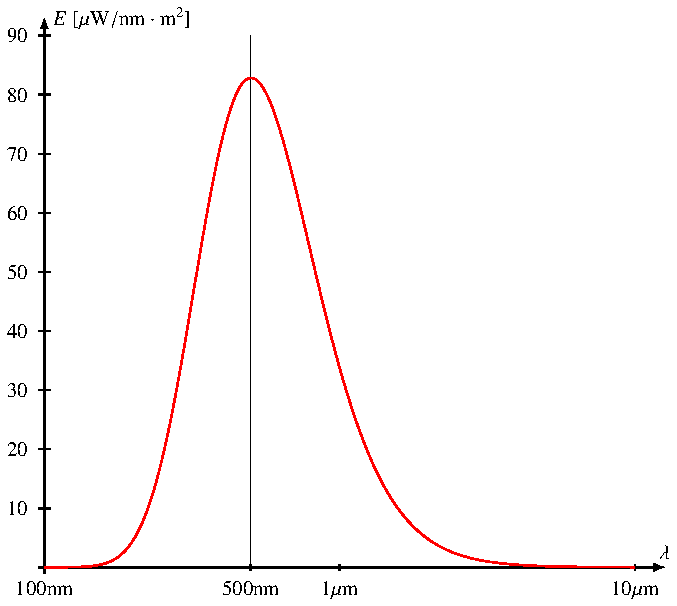
\includegraphics{chapters/1/planck.pdf}
\caption{Plancksches Strahlungsgesetz für die Sonne
\label{skript:planck-kurve}}
\end{figure}
\index{Plancksches Strahlungsgesetz}
\index{Strahlungsgesetz,Plancksches}
Die Strahlungsdichte in Abhängigkeit von der Wellenlänge ist in
Abbildung~\ref{skript:planck-kurve} dargestellt.
Die gesamte Strahlungsleistung ist das Integral
\[
P
=
\int_{0}^\infty E(\lambda,T)\,d\lambda
=
\int_{0}^\infty 
\frac{2\pi hc^2}{\lambda^5}\frac{d\lambda}{e^{\frac{hc}{\lambda kT}}-1}.
\]

\subsubsection{Einstrahlungswinkel}
Warum ist es in den Tropen wärmer als in gemässigten Breiten oder
an den Polen?
Die Sonne strahlt doch überall mit der gleichen Intensität.

Der Unterschied ist natürlich der Einstrahlungswinkel.
Der Ausdruck \eqref{skript:solarkonstante} für $P_{\earth}$ 
beschreibt die Strahlungsleistung pro Flächeneinheit, doch diese
Flächeneinheit wird senkrecht auf die Ausbreitungsrichtung der
Strahlung gemessen.
In gemässigten Breiten und an den Polen fällt die Strahlung 
in viel kleinerem Winkel auf die Erdoberfläche.
Die einfallende Energie verteilt sich daher auf eine grössere
Fläche.
Ist $\alpha$ der Winkel zwischen der Vertikalen und der Strahlungsrichtung,
dann ist die auf einer Erdoberfläche einfallende Strahlungsdichte nur
noch $P_{\earth}\cdot\cos\alpha$.

\begin{figure}
\centering
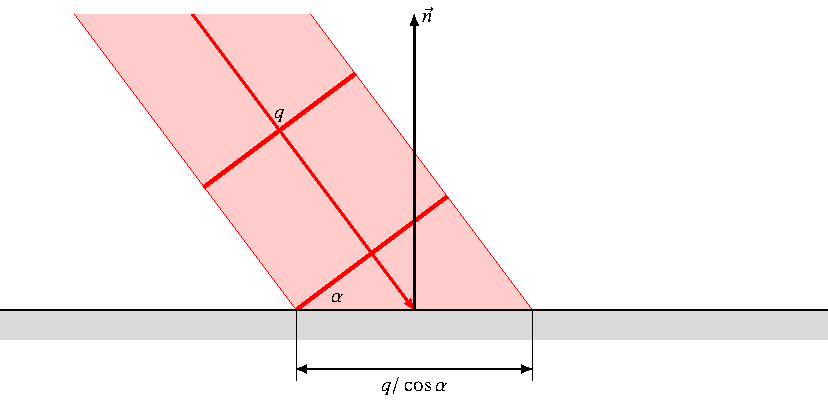
\includegraphics{chapters/1/einfall.pdf}
\caption{Einfluss des Einstrahlungswinkels auf die pro Flächeneinheit
der Erdoberfläche einfallende Strahlungsleistung.
Ein Strahlenbündel mit Querschnitt $q$, welches im Winkel
$\alpha$ zur Vertikalen einfällt, bedeckt die Fläche $q/\cos\alpha$
auf der Erdoberfläche
\label{skript:einfallswinkel}}
\end{figure}
Man beachte aber, dass in den graphischen Darstellungen des
Strahlungsspektrums eine logarithmische $\lambda$-Skala
verwendet wird.
Bei grossen Wellenlängen (``rechts'') wird die Kurve also in Wahrheit
viel stärker ausgedehnt.
Will man die Flächeninhalte unter den Kurven vergleichen, muss man
die veritkale Achse mit dem Faktor $\lambda$ skalieren.

\subsubsection{Strahlungsbilanz}
\begin{figure}
\centering
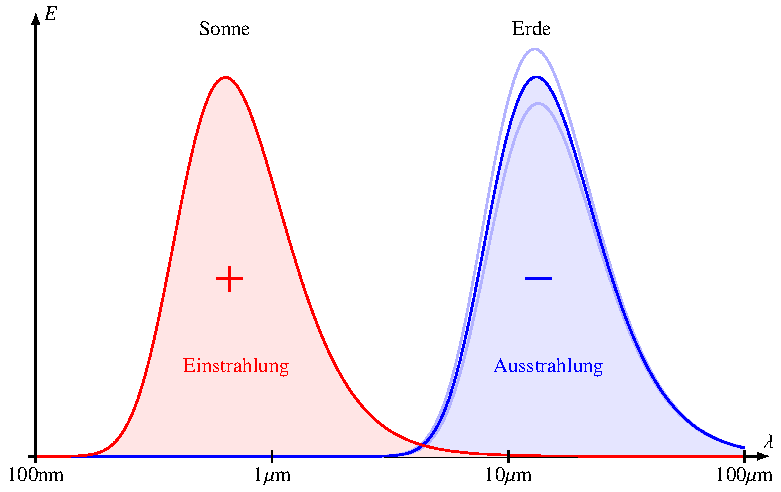
\includegraphics{chapters/1/vergleich.pdf}
\caption{Strahlung der Sonne (rot) und der Erde (blau).
Das Maximum der Strahlung der Sonne ist im sichtbaren Bereich,
das Maximum der Wärmestrahlung der Erde im Infraroten.
\label{skript:strahlung-sonne-erde}}
\end{figure}%
In Abbildung~\ref{skript:strahlung-sonne-erde} sind die Planckschen
Strahlungskurve für die Sonne und Erde dargestellt.
Die rote Kurve zeigt die spektrale Strahlungsleistung, die von der
Sonne auf den Querschnitt $\pi R_{\earth}^2$ der Erde eingestrahlt wird,
also
\[
E(\lambda,T_{\astrosun}) \cdot 2\pi R_{\earth}^2
\cdot
\biggl(\frac{R_{\astrosun}}{a_{\earth}}\biggr)^2
\]
mit $T_{\astrosun}=5778\text{K}$.
Die dunkelblaue Kurve zeigt das Ausstrahlungsspektrum der ganzen Erde mit
einer Temperatur von $T=279\text{K}$, also
\[
E(\lambda,T_{\earth})\cdot 4\pi R_{\earth}^2.
\]
Die Fläche unter der Kurve ist ein Mass für die gesamte Energie.
Offenbar halten sich Einstrahlung und Ausstrahlung die Waage.

Die Einstrahlung kann sich zum Beispiel dann verändern, wenn 
mehr Strahlung reflektiert wird.
Die Ausstrahlung verändert sich, wenn die Atmosphäre für infrarote
Strahlung grösser wird.
Wir die Atmosphäre durch erhöhte $\text{CO}_2$-Konzentration für
infrarote Strahlung undurchsichtiger, dann sinkt die Ausstrahlung
der Erde.
Damit wieder ein Gleichgewicht entsteht, muss die Temperatur der
Erde sich erhöhen, damit die Ausstrahlung ebenfalls höher wird
(obere hellblaue Kurve).
Sinkt der Gehalt an Treibhausgasen, wird die Atmosphäre transparenter
für Wärmestrahlung.
Ein Gleichgewicht ist möglich bei tieferer Temperatur (untere
hellblaue Kurve).
Diese Abhängigkeit der Temperatur von der Transparenz der
Atmosphäre für Wärmestrahlung ist bekannt als der {\em Treibhauseffekt}.
\index{Treibhauseffekt}

\subsubsection{Tatsächliches Strahlungspektrum}
\begin{figure}
\centering
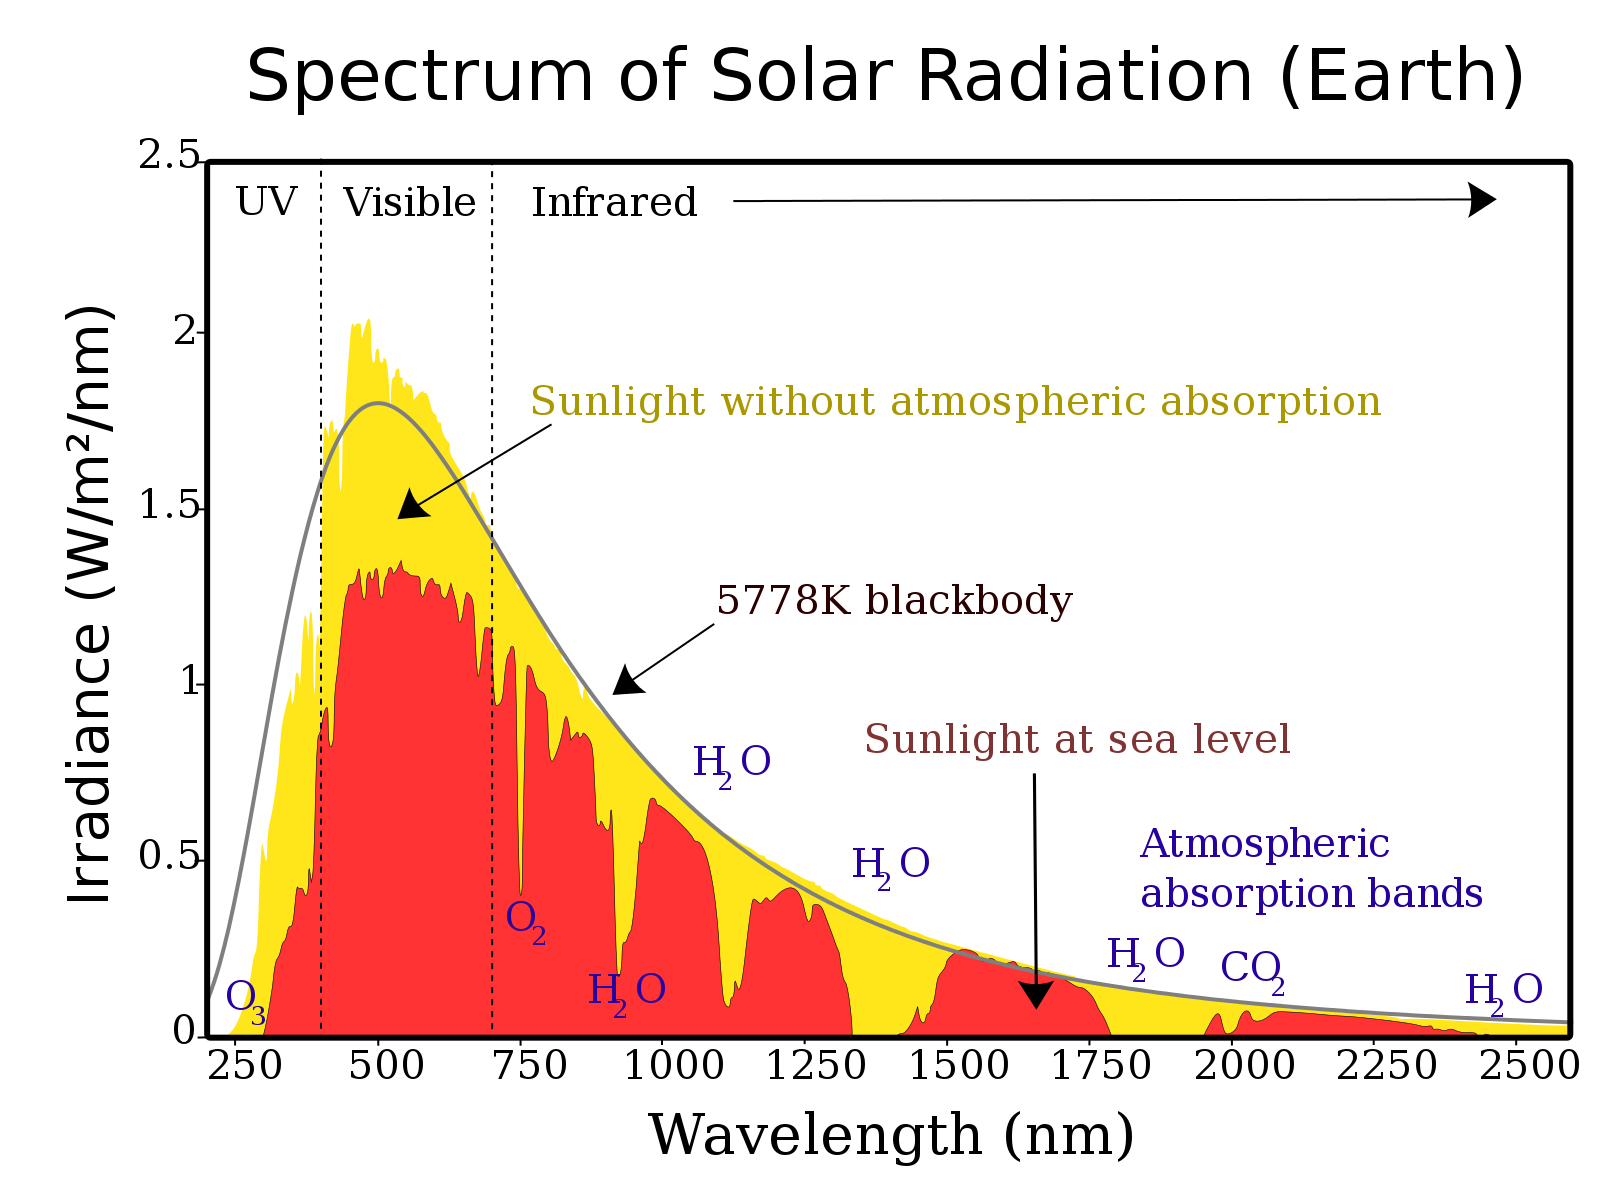
\includegraphics[width=0.7\hsize]{chapters/1/Solar_spectrum_en.png}
\caption{Tatsächliches Spektrum der Sonnenstrahlung mit (rot) und
ohne (gelb) atmosphärische Absorbtion im Vergleich mit dem Spektrum
der Schwarzkörperstrahlung \cite{skript:sunlight}.
\label{skript:strahlungsspektrum}}
\end{figure}
In Abbildung~\ref{skript:strahlungsspektrum} ist das tatsächlich gemessene
Strahlungsspektrum der Sonne dargestellt.
Es fällt auf, dass Wasserdampf und $\text{CO}_2$  für bedeutende
Absorbtionsbänder verantwortlich ist, während im sichtbaren bereich
die Absorbtion sehr gleichmässig ist.

\subsection{Erdrotation und Zirkulation}
Die Einstrahlung ist naturgemäss am grössten am Äquator, während am 

\subsubsection{Coriolis-Effekt}
\index{Coriolis-Kraft}%
\index{Coriolis-Effekt}%
\subsubsection{Globale Zirkulation}
\subsubsection{Äquatorialzone}

\subsection{Periodische Einflüsse}
Das Klimasystem ist einer Reihe von sich periodisch verändernden 
Einflüssen ausgesetzt.
Viele dieser Einflüsse erscheinen auf den ersten Blick geringfügig
und damit vernachlässigbar.
Doch wenn ein solcher periodischer Einfluss mit einer Frequenz auftritt,
der einer Eigenfrequenz des Klimasystems entspricht, dann kann sich 
in Folge eines Resonanzeffektes über längere Zeit ein bedeutender 
Einfluss auf das Klima manifestieren.
Es ist daher wichtig, auch kleine Einflüsse zu kennen und insbesondere
alle Aspekte des Klimasystems zu modellieren, die eine Eigenfrequenz
in der Nähe ihrer Anregungsfrequenzen haben.

\subsubsection{Sonnenfleckenzyklus}
\index{Sonnenflecken}%
\index{Sonnenfleckenzyklus}%
Die Strahlung der Sonne ist nicht konstant.
Wie bei jedem Stern dieser Klasse nehmen Durchmesser und Temperatur der
Sonne über die Jahrmillionen in dem Mass zu, dass neben der Fusion
von Wasserstoff zu Helium auch noch Fusionsprozesse schwerer Elemente
eine Rolle zu spielen beginnen.
Dieser sehr langfristige Einfluss ist jedoch nur wesentlich für
den Vergleich von Klimamodellen mit Daten über das Klima auf der sehr
jungen Erde.

Für kurzfristige Prognosen von Bedeutung sind dagegen die Schwankungen
der Sonnenaktivität.
\index{Sonnenaktivität}%
Die Zahl der Sonnenflecken ist ein leicht zu messender Indikator
dafür, für den Aufzeichnung seit dem 17.~Jahrhundert existieren.
Die Sonnenfleckenzahl schwankt mit einer Periode von etwa elf Jahren.
Die daraus resultierende Änderung der Einstrahlung ist jedoch nur 0.07\%,
so dass die Sonnenaktivität nicht für den Klimawandel verantwortlich
gemacht werden kann. 
Die schwankende Sonnenaktivität muss jedoch bei der Validierung
von Klimamodellen berücksichtigt werden.

\subsubsection{Bahnänderungen der Erde}
\index{Bahnänderungen}%
Nach Kepler bewegen sich die Planeten auf Ellipsen,
in deren einem Brennpunkt die Sonne steht.
Die keplerschen Gesetze der Planetenbahnen können aus dem Newtonschen 
Gravitationsgesetz hergeleitet werden
\cite[\S 6]{skript:joos}.
\index{Bahnelemente}%
\index{Keplersche Gesetze}
Die Bahnelemente beschreiben die Ebene, in der sich der Planet bewegt,
die Richtung und der Zeitpunkt der grössten Annäherung an die Sonne und
die Exzentrizität der Ellipse.
\index{Exzentrizität}%

Es trifft exakt jedoch nur dann zu, wenn keine anderen Kräfte auf den
Planeten wirken als die Anziehungskraft der Sonne.
Newtons Gravitationsgesetzt besagt jedoch, dass auch alle anderen
Planeten durch ihre Schwerkraft auf die Erde einwirken.
Dies äussert sich darin, dass die Bahnelemente, sich mit der Zeit
ändern.
Diese langsame Veränderung der Bahnelemente war schon Newton bekannt,
er hat daraus geschlossen, dass das Sonnensystem mit der Zeit völlig
zerfallen würde.
Genauere Untersuchungen und numerische Rechnungen zeigen jedoch, dass
unser Sonnensystem über lange Zeit stabil ist.
Die Exzentrizität zum Beispiel der Erdbahn kann sich tatsächlich verändern,
aber über längere Zeit wird die Veränderung auch wieder rückgängig
gemacht.

Veränderungen der Erdbahn, insbesondere der Exzentrizität, oder der
Neigung der Erdachse zur Bahn äussern sich darin, dass die Einstrahlung
über das Jahr stärker oder weniger stark schwankt oder auch im Mittel
grösser oder kleiner wird.
\index{Neigung der Erdachse}%
Dadurch können sich die Temperaturunterschiede zwischen den Polgebieten und
äquatorialen Breiten verändern und damit die Intensität des Wettergeschehens
beeinflusst werden.
Ein langfristiges Klimamodell muss also auch diese Änderungen
modellieren.

Es stellt sich allerdings heraus, dass diese Veränderungen sehr viel
langfristiger sind als der die meisten Klimapolitiker interessierenden
Zeitraum von wenigen Jahrhunderten.
Die Berücksichtigung dieser Effekte dient daher vor allem dazu die
Klima-Modelle mit der Klimageschichte der Erde zu vergleichung und
damit zu validieren.
In Kapitel~\ref{chapter:fourier} wird gezeigt, wie periodische Einflüsse
modelliert und mit Hilfe der Fourier-Theorie analysiert werden können.

